\documentclass[11pt]{article}
\title{Meccano triangles}
\author{https://github.com/heptagons/meccano/nest}
\date{}

\newfam\bbbfam
\font\bbbten=msbm10
\font\bbbseven=msbm7
\font\bbbfive=msbm5
\textfont\bbbfam=\bbbten
\scriptfont\bbbfam=\bbbseven
\scriptscriptfont\bbbfam=\bbbfive
\def\bbb{\fam=\bbbfam}

\usepackage{../../meccano}
\begin{document}

\maketitle
\begin{abstract}
We construct meccano triangles. Basic triangles has the three sides as integers and calculate the internal diagonal distances.
Such diagonals then are used as the new side of more complicated triangles and then again we
calculate new distances formed and so on. Eventually we expect to
find certain angles joining the triangles which can be used to construct regular polygons or more figures.
\end{abstract}

\section{Triangles $(a,b,c)$}
Triangles $(a,b,c)$ have three sides $a$, $b$ and $c$ where $a, b, c \in \bbb N$.
To avoid repetitions and get only valid triangles, we consider only the cases:
\begin{align}
a &\ge b \ge c\\
a &< b + c
\end{align}
We calculate the three angles cosines. The three cosines are rationals:
\begin{align}
\cos{A} &= \frac{b^2 + c^2 - a^2}{2bc} &\in \bbb Q\\
\cos{B} &= \frac{c^2 + a^2 - b^2}{2ca} &\in \bbb Q\\
\cos{C} &= \frac{a^2 + b^2 - c^2}{2ab} &\in \bbb Q
\end{align}

\subsection{Triangle $(a,b,c)$ diagonals}

To calculate the diagonals we use the law of cosines.
With the $\cos{A}$ we can calculate every diagonal $\overline{b_mc_n}$ with:
\begin{align}
\overline{b_mc_n} &= \sqrt{m^2 + n^2 - 2mn\cos{A}}\\
       &= \sqrt{m^2 + n^2 - 2mn\frac{b^2 + c^2 - a^2}{2bc}}\\
       &= \frac{\sqrt{b^2c^2(m^2 + n^2)-bcmn(b^2 + c^2 - a^2)}}{bc} &\in \bbb A
\end{align}
where $1 \le m \le b$, $1 \le n \le c$ and $m - n \ge 0$. Similarly:
\begin{align}
\overline{c_ma_n} &= \frac{\sqrt{c^2a^2(m^2 + n^2)-camn(c^2 + a^2 - b^2)}}{ac} &\in \bbb A\\
\overline{a_mb_n} &= \frac{\sqrt{a^2b^2(m^2 + n^2)-abmn(a^2 + b^2 - c^2)}}{ab} &\in \bbb A
\end{align}
The diagonals are algebraic of the form $\frac{y\sqrt{z}}{x}$.

\subsection{Example triangle (7,6,5)}

\begin{figure}[htp]
\centering
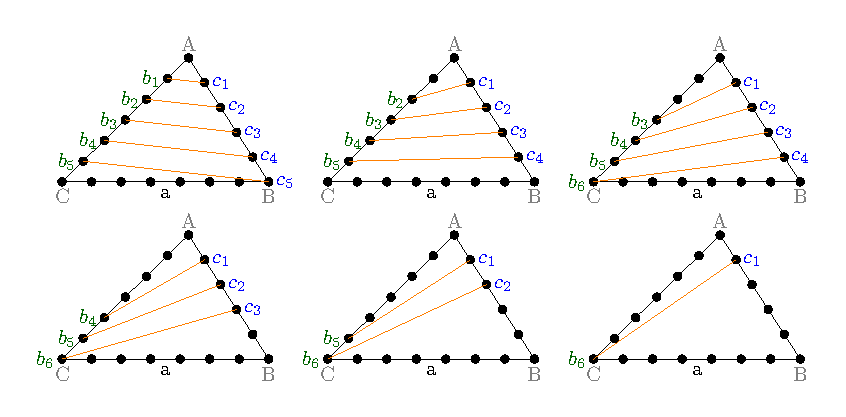
\includegraphics[scale=1]{t765bc}
\caption{Triangle $(7,6,5)$ $b_mc_n$ diagonals ($m \ge n$).
For top to bottom and left to right we have six groups of diagonals.
Each group is defined by $m$ and $n$ indices difference:
$m - n = 0$, $m - n = 1$, ... $m - n = 5$.
}
\label{t765bc}
\end{figure}

\begin{figure}[htp]
\centering
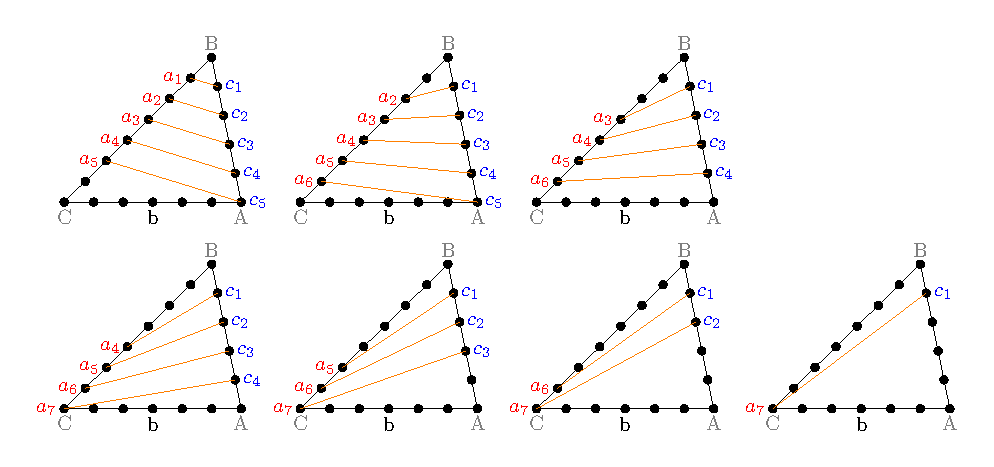
\includegraphics[scale=1]{t765ac}
\caption{Triangle $(7,6,5)$, $a_mc_n$ diagonals ($m \ge n$).
We have also six group. But here we found diagonals repetead already
found in previous figure. Diagonals repeated are all including $a_7$ points.
}
\label{t765ac}
\end{figure}

\begin{figure}[htp]
\centering
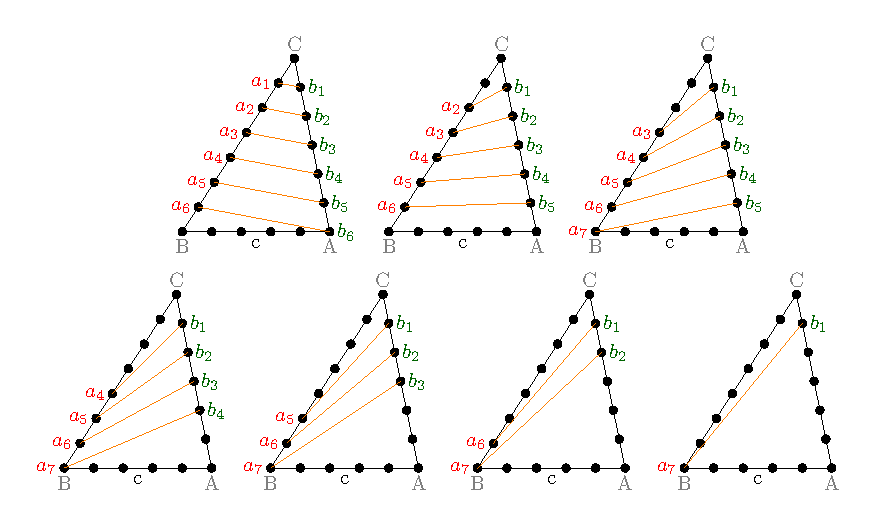
\includegraphics[scale=1]{t765ab}
\caption{Triangle $(7,6,5)$, $a_mb_n$ diagonals ($m \ge n$).
Here we have diagonals repeteated already in previous figure.
Using matrices we can reject such diagonals rejecting matrices columns.
}
\label{t765ab}
\end{figure}

\newcommand\five{\colorbox{green}{$5$}}

Figure \ref{t765bc} show triangle $(7,6,5)$ diagonals $b_mc_n$ for vertex $A$. For this figure we calculate
the values and form a matrix. Empty cells are reflections:
\begin{equation}\label{eq:appendrow}
\left(\begin{array}{cccccc}
	\frac{2\sqrt{10}}{5} & \frac{\sqrt{105}}{5} & \frac{2\sqrt{55}}{5} & \frac{\sqrt{385}}{5} & 2\sqrt{6} & \frac{\sqrt{865}}{5} \\
	& \frac{4\sqrt{10}}{5} & \frac{\sqrt{265}}{5} & \frac{2\sqrt{105}}{5} & \five & \frac{4\sqrt{55}}{5} \\
	& & \frac{6\sqrt{10}}{5} & \frac{\sqrt{505}}{5} & 2\sqrt{7} & \frac{3\sqrt{105}}{5}\\
	& & & \frac{8\sqrt{10}}{5} & \sqrt{33} & \frac{2\sqrt{265}}{5}\\
	& & & & 2\sqrt{10} & \boxed{7} \\
\end{array}\right)
\end{equation}

Figure \ref{t765ac} show triangle $(7,6,5)$ diagonals $a_mc_n$ for vertex $B$. For this figure we calculate
the values for a second matrix. Values at column 7 (at the right of separator $|$) are repeated and already in previous matrix.
Empty cells are reflections.
\begin{equation}\label{eq:appendrow}
\left(\begin{array}{cccccccc}
	\frac{4\sqrt{70}}{35} & \frac{3\sqrt{385}}{35} & \frac{2\sqrt{2065}}{35} & \frac{\sqrt{15505}}{35} & \frac{12\sqrt{7}}{7} & \frac{\sqrt{37345}}{35} & | & \frac{2\sqrt{265}}{5}\\
	& \frac{8\sqrt{70}}{35} & \frac{\sqrt{7945}}{35} & \frac{6\sqrt{385}}{35} & \frac{\sqrt{889}}{7} & \frac{4\sqrt{2065}}{35} & | & \frac{3\sqrt{105}}{5} \\
	& & \frac{12\sqrt{70}}{35} & \frac{\sqrt{14665}}{35} & \frac{2\sqrt{217}}{7} & \frac{9\sqrt{385}}{35} & | & \frac{4\sqrt{55}}{5}\\
	& & & \frac{16\sqrt{70}}{35} & \frac{3\sqrt{105}}{7} & \frac{2\sqrt{7945}}{35} & | & \frac{\sqrt{865}}{5}\\
	& & & & \frac{4\sqrt{70}}{7} & \frac{\sqrt{1393}}{7} & | & \boxed{6}\\
\end{array}\right)
\end{equation}

Figure \ref{t765ab} show triangle $(7,6,5)$ diagonals $a_mb_n$ for vertex $C$. For this figure we calculate
the values for a third matrix. Values at columns 6 and 7 (at the right of separator $|$) 
are repeated and already in previous matrices.
\begin{equation}\label{eq:appendrow}
\left(\begin{array}{cccccccc}
	\frac{2\sqrt7}7 & \frac{\sqrt{105}}7 & \frac{2\sqrt{70}}7 & \frac{\sqrt{553}}7 & \frac{2\sqrt{231}}7 & | &  \frac{\sqrt{1393}}7 & 2\sqrt{10} \\
	 & \frac{4\sqrt7}7 & \frac{\sqrt{217}}7 & \frac{2\sqrt{105}}7 & \frac{\sqrt{721}}7 & | &  \frac{4\sqrt{70}}7 & \sqrt{33} \\
	 & & \frac{6\sqrt7}7 & \frac{\sqrt{385}}7 & \frac{2\sqrt{154}}7 & | &  \frac{3\sqrt{105}}7 & 2\sqrt{7} \\
	 & & & \frac{8\sqrt7}7 & \frac{\sqrt{609}}7 & | &  \frac{2\sqrt{217}}7 & \five \\
	 & & & & \frac{10\sqrt7}7 & | &  \frac{\sqrt{889}}7 & 2\sqrt{6} \\
	 & & & & & | & \frac{12\sqrt7}7 & \boxed{5} \\
\end{array}\right)
\end{equation}

\section{Triangles$(\sqrt{\alpha},b,c)$}

Triangles$(\sqrt{\alpha},b,c)$ have three sides with lengths $a=\sqrt{\alpha}$, $b$ and $c$ where $\alpha, b, c \in \bbb N$
and $\alpha$ is squarefree. We have:
\begin{align}
\sqrt{\alpha} &> b \ge c &\implies \alpha  > b^2 \ge c^2 \\
\sqrt{\alpha} &< b + c   &\implies \alpha < (b + c)^2
\end{align}
We calculate the triangle cosines. $\cos{A}$ is rational and $\cos{B}$ and $\cos{C}$ are algebraic:
\begin{align}
\cos{A} &= \frac{b^2 + c^2 - (\sqrt{\alpha})^2}{2bc} = \frac{b^2 + c^2 - \alpha}{2bc} &\in \bbb{Q} \\
\cos{B} &= \frac{(\sqrt{\alpha})^2 + c^2 - b^2}{2\sqrt{\alpha}c} = \frac{(\alpha + c^2 - b^2)\sqrt{\alpha}}{2\alpha c} &\in \bbb{A} \\
\cos{C} &= \frac{(\sqrt{\alpha})^2 + b^2 - c^2}{2\sqrt{\alpha}b} = \frac{(\alpha + b^2 - c^2)\sqrt{\alpha}}{2\alpha b} &\in \bbb{A} 
\end{align}

\subsection{Triangle $(\sqrt{\alpha},b,c)$ diagonals}

The only possible diagonals are for sides with integers, that is $\overline{b_mc_n}$. Using the law of cosines:
\begin{align}
\overline{b_mc_n} &= \sqrt{m^2 + n^2 - 2mn\cos{A}}\\
  &= \sqrt{m^2 + n^2 - 2mn\frac{b^2 + c^2 - \alpha}{2bc}}\\
  &= \frac{\sqrt{b^2c^2(m^2 + n^2)-bcmn(b^2 + c^2 - \alpha)}}{bc} &\in \bbb{A}
\end{align}
where $1 \le m \le b$, $1 \le n \le c$ and $m \ge n$.

\subsection{Example triangles$(2\sqrt{6},b,c)$}

In this case $\sqrt{\alpha} = 2\sqrt{6}$ so $\alpha = 24$.
Then $m = n = \{ 1,2,3,4 \}$ because $b^2 = c^2 = \{ 1,4,9,16\} < 24$.
We form a matrix with the values $(b+c)^2$ and satisfying $b \ge c$:
\begin {equation}\label{E:2}
(b_m + c_n)^2 =\bordermatrix{~ & b=1 & b=2 & b=3 & b=4 \cr
c=1 &  2 &  9 & 16 & 25 \cr    
c=2 & \times & 16 & 25 & 36 \cr    
c=3 & \times & \times & 36 & 49 \cr    
c=4 & \times & \times & \times & 64 \cr}
\end {equation}

Then we remove the cells that don't satisfy the condition $\alpha < (b+c)^2$:
\begin {equation}\label{E:3}
(b_m + c_n)^2 =\bordermatrix{~ & b=1 & b=2 & b=3 & b=4 \cr
c=1 & \times & \times & \times & 25 \cr    
c=2 & & \times & 25 & 36 \cr    
c=3 & & & 36 & 49 \cr    
c=4 & & & & 64 \cr}
\end {equation}

\begin{figure}[htp]
\centering
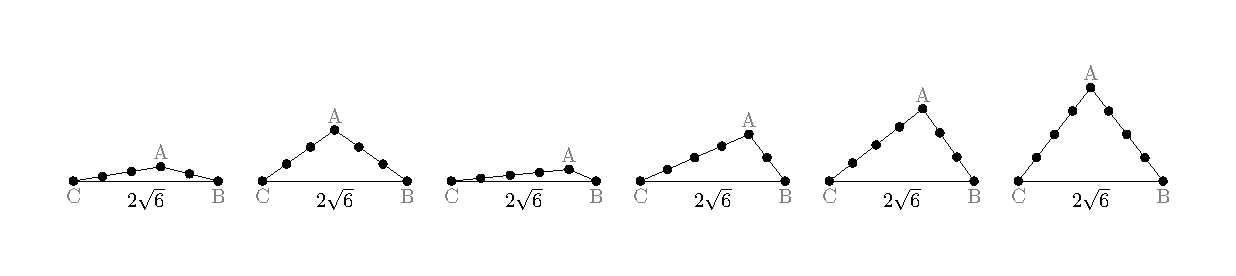
\includegraphics[scale=0.9]{tslurA}
\caption{All triangles with sides $a = 2\sqrt{6} > b \ge c$}
\label{tslurA}
\end{figure}
    
Each remaining cell in the matrix corresponds to a particular triangle:
\begin {equation}\label{E:4}
(2\sqrt{6},b,c) =\bordermatrix{~ & \cos{A} & \cos{B} & \cos{C} \cr
(2\sqrt{6},3,2) & -\frac{11}{12} & \frac{19\sqrt{6}}{48} & \frac{29\sqrt{6}}{72} \cr
(2\sqrt{6},3,3) & -\frac{1}{3}   & \frac{\sqrt{6}}{3}    & \frac{\sqrt{6}}{3}    \cr
(2\sqrt{6},4,1) & -\frac{7}{8}   & \frac{3\sqrt{6}}{8}   & \frac{13\sqrt{6}}{32} \cr
(2\sqrt{6},4,2) & -\frac{1}{4}   & \frac{\sqrt{6}}{4}    & \frac{3\sqrt{6}}{8}   \cr
(2\sqrt{6},4,3) &  \frac{1}{24}  & \frac{17\sqrt{6}}{72} & \frac{31\sqrt{6}}{96} \cr
(2\sqrt{6},4,4) &  \frac{1}{4}   & \frac{\sqrt{6}}{4}    & \frac{\sqrt{6}}{4}    \cr}
\end{equation}

Figure \ref{tslurA} show the triangles $(2\sqrt{6},b,c)$. The cosines are calculated by code at:
\\\\
\texttt{github.com/heptagons/meccano/nest/t\_test.go TestTslursA}

\section{Triangles$(a,\sqrt{\beta},c)$}

Triangles$(a,\sqrt{\beta},c)$ have the three sides $a$, $b = \sqrt{\beta}$ and $c$ where $a, \beta, c \in \bbb N$ and $\beta$ is squarefree.
We have:
\begin{align}
a &> \sqrt{\beta} > c &\implies a^2 > \beta > c^2 \\
a &< \sqrt{\beta} + c &\implies (a-c)^2 < \beta
\end{align}
We calculate the triangle cosines. $\cos{A}$ is algebraic, $\cos{B}$ rational and $\cos{C}$ algebraic:
\begin{align}
\cos{A} &= \frac{(\sqrt{\beta})^2 + c^2 - a^2}{2\sqrt{\beta}c} = \frac{(\beta + c^2 - a^2)\sqrt{\beta}}{2\beta c} &\in \bbb{A} \\
\cos{B} &= \frac{a^2 + c^2 - (\sqrt{\beta})^2}{2ac} = \frac{a^2 + c^2 - \beta}{2ac} &\in \bbb{Q} \\
\cos{C} &= \frac{a^2 + (\sqrt{\beta})^2 - c^2}{2a\sqrt{\beta}} = \frac{(a^2 + \beta - c^2)\sqrt{\beta}}{2a\beta} &\in \bbb{A} 
\end{align}

\subsection{Triangle $(a, \sqrt{\beta},c)$ diagonals}

The only possible diagonals are for sides with integers, that is $\overline{a_mc_n}$. Using the law of cosines:
\begin{align}
\overline{a_mc_n} &= \sqrt{m^2 + n^2 - 2mn\cos{B}}\\
  &= \sqrt{m^2 + n^2 - 2mn\frac{a^2 + c^2 - \beta}{2ac}}\\
  &= \frac{\sqrt{a^2c^2(m^2 + n^2)-acmn(a^2 + c^2 - \beta)}}{ac} &\in \bbb{A}
\end{align}
where $1 \le m \le a$, $1 \le n \le c$ and $m \ge n$.

\subsection{Example triangles$(a,2\sqrt{6},c)$}

In this case $\sqrt{\beta} = 2\sqrt{6}$ so $\beta = 24$. 
Then $m = \{ 5,6,7,... \}$ because $m^2 = \{ 25,36,49,... \} > 24$ and
$n = \{ 1,2,3,4 \}$ because $c^2 = \{ 1,4,9,16\} < 24$.
We form a matrix with the values $(a-c)^2$:
\begin {equation}\label{E:11}
(a_m - c_n)^2 =\bordermatrix{~ & a=5 & a=6 & a=7 & a=8 & a=9 & ...\cr
c=1 & 16 & 25 & 36 & 49 & 64 & ...\cr    
c=2 &  9 & 16 & 25 & 36 & 49 & ...\cr    
c=3 &  4 &  9 & 16 & 25 & 36 & ...\cr    
c=4 &  1 &  4 &  9 & 16 & 25 & ...\cr}
\end {equation}

We remove cells which don't satisfy the condition $(a-c)^2 < \beta$:
\begin {equation}\label{E:12}
(a_m - c_n)^2 =\bordermatrix{~ & a=5 & a=6 & a=7 & a=8 & a=9 & ...\cr
c=1 & 16 & \times & \times & \times & \times & ...\cr    
c=2 &  9 & 16 & \times & \times & \times & ...\cr    
c=3 &  4 &  9 & 16 & \times & \times & ...\cr    
c=4 &  1 &  4 &  9 & 16 & \times & ...\cr}
\end {equation}

\begin{figure}[htp]
\centering
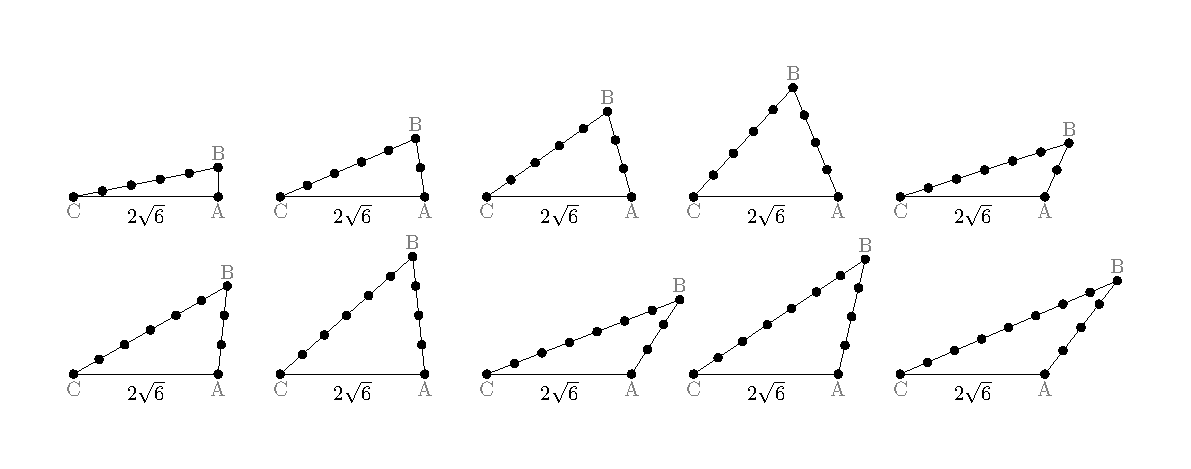
\includegraphics[scale=0.9]{tslurB}
\caption{All triangles with sides $a > b = 2\sqrt{6} > c$}
\label{tslurB}
\end{figure}

So we have ten triangles are valid:
\begin {equation}\label{E:13}
(a,2\sqrt{6},c) =\bordermatrix{~ & \cos{A} & \cos{B} & \cos{C} \cr
(5,2\sqrt{6},1) & 0         & \frac{1}{5} & \frac{2\sqrt{6}}{5} \cr
(5,2\sqrt{6},2) & \frac{\sqrt{6}}{16} & \frac{1}{4} & \frac{3\sqrt{6}}{8} \cr
(5,2\sqrt{6},3) & \frac{\sqrt{6}}{9} & \frac{1}{3} & \frac{\sqrt{6}}{3} \cr
(5,2\sqrt{6},4) & \frac{5\sqrt{6}}{32} & \frac{17}{40} & \frac{11\sqrt{6}}{40} \cr
(6,2\sqrt{6},2) & \frac{\sqrt{6}}{6} & \frac{2}{3} & \frac{7\sqrt{6}}{18} \cr
(6,2\sqrt{6},3) & \frac{\sqrt{6}}{24} & \frac{7}{12} & \frac{17\sqrt{6}}{48} \cr
(6,2\sqrt{6},4) & \frac{\sqrt{6}}{24} & \frac{7}{12} & \frac{11\sqrt{6}}{36} \cr
(7,2\sqrt{6},3) & -\frac{2\sqrt{6}}{9} & \frac{17}{21} & \frac{8/sqrt{6}}{21} \cr
(7,2\sqrt{6},4) & -\frac{3\sqrt{6}}{32} & \frac{41}{56} & \frac{19\sqrt{6}}{56} \cr
(8,2\sqrt{6},4) & \frac{\sqrt{6}}{4} & \frac{7}{8} & \frac{3\sqrt{6}}{8} \cr}
\end{equation}

Figure \ref{tslurB} show the triangles $(a,2\sqrt{6},c)$. The cosines are calculated by code at:
\\\\
\texttt{github.com/heptagons/meccano/nest/t\_test.go TestTslursB}


\section{Triangles$(a,b,\sqrt{\gamma})$}

Triangles$(a,b,\sqrt{\gamma})$ have three sides $a$, $b$, $\sqrt{\gamma}$ where $a, b, \gamma \in \bbb N$ and $\gamma$ is squarefree.
We have:
\begin{align}
a &\ge b > \sqrt{\gamma} &\implies a^2 \ge b^2 > \gamma \\
a &< b + \sqrt{\gamma} &\implies (a-b)^2 < \gamma
\end{align}
We calculate the triangle cosines. $\cos{A}$ and $\cos{B}$ are algebraic and $\cos{C}$ rational:
\begin{align}
\cos{A} &= \frac{b^2 + \gamma - a^2}{2b\sqrt{\gamma}} = \frac{(b^2 + \gamma - a^2)\sqrt{\gamma}}{2b\gamma} &\in \bbb{A} \\
\cos{B} &= \frac{a^2 + \gamma - b^2}{2a\sqrt{\gamma}} = \frac{(a^2 + \gamma - b^2)\sqrt{\gamma}}{2a\gamma} &\in \bbb{A} \\
\cos{C} &= \frac{a^2 + b^2 - (\sqrt{\gamma})^2}{2ab} = \frac{a^2 + b^2 - \gamma}{2ab} &\in \bbb{Q} 
\end{align}

\subsection{Triangle $(a, b, \sqrt{\gamma})$ diagonals}

The only possible diagonals are for sides with integers, that is $\overline{a_mb_n}$. Using the law of cosines:
\begin{align}
\overline{a_mb_n} &= \sqrt{m^2 + n^2 - 2mn\cos{C}}\\
  &= \sqrt{m^2 + n^2 - 2mn\frac{a^2 + b^2 - \gamma}{2ab}}\\
  &= \frac{\sqrt{a^2b^2(m^2 + n^2)-acmn(a^2 + b^2 - \gamma)}}{ab} &\in \bbb{A}
\end{align}
where $1 \le m < a$, $1 \le n < b$ and $m \ge n$.

\subsection{Example triangles$(a,b,2\sqrt{6})$}

In this case $\sqrt{\gamma} = 2\sqrt{6}$ so $\gamma = 24$. 
We form a matrix with with the values $(a-b)^2$ satisfying the condition $a^2 \ge b^2 > \gamma$:
\begin {equation}\label{E:21}
(a_m - b_n)^2 =\bordermatrix{~ & a=5 & a=6 & a=7 & a=8 & a=9 & a=10 & a=11 & a=12 & \hdots\cr
b=5  & 0 & 1 & 4 &  9 & 16 & 25 & 36 & 49 & \hdots \cr    
b=6  &   & 0 & 1 &  4 &  9 & 16 & 25 & 36 & \hdots \cr    
b=7  &   &   & 0 &  1 &  4 &  9 & 16 & 25 & \hdots \cr    
b=8  &   &   &   &  0 &  1 &  4 &  9 & 16 & \hdots \cr    
b=9  &   &   &   &    &  0 &  1 &  4 &  9 & \hdots \cr    
b=10 &   &   &   &    &    &  0 &  1 &  4 & \hdots \cr    
 &  &  &  &  &  & \vdots & \vdots & \vdots & \ddots \cr}
\end {equation}

We remove cells except those satisfying the condition $(a-b)^2 < \gamma$:
\begin {equation}\label{E:21}
(a_m - b_n)^2 =\bordermatrix{~ & a=5 & a=6 & a=7 & a=8 & a=9 & a=10 & a=11 & a=12 & \hdots\cr
b=5  & 0 & 1 & 4 &  9 & 16 & \times & \times & \times & \hdots \cr    
b=6  &   & 0 & 1 &  4 &  9 & 16 & \times & \times & \hdots \cr    
b=7  &   &   & 0 &  1 &  4 &  9 & 16 & \times & \hdots \cr    
b=8  &   &   &   &  0 &  1 &  4 &  9 & 16 & \hdots \cr    
b=9  &   &   &   &    &  0 &  1 &  4 &  9 & \hdots \cr    
b=10 &   &   &   &    &    &  0 &  1 &  4 & \hdots \cr    
 &  &  &  &  &  & \vdots & \vdots & \vdots & \ddots \cr}
\end {equation}

\begin{figure}[htp]
\centering
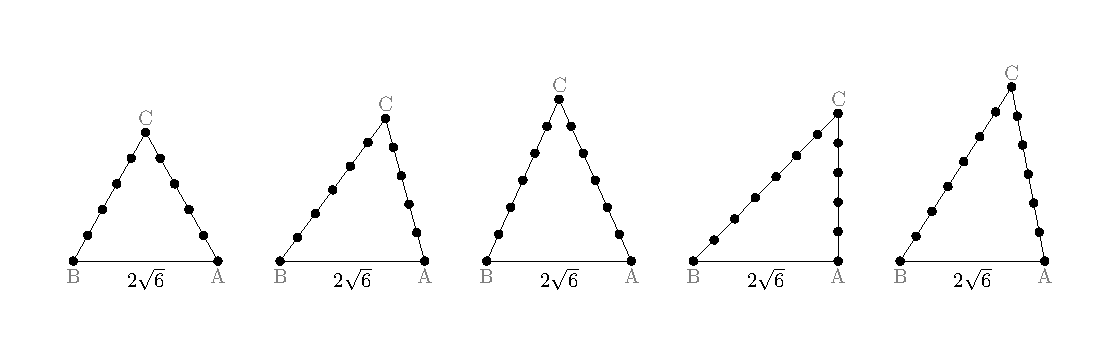
\includegraphics[scale=0.9]{tslurC}
\caption{Some triangles with sides $a \ge b > c = 2\sqrt{6}$}
\label{tslurC}
\end{figure}

So we found that infinite triangles are valid, the smaller ones are:
\begin {equation}\label{E:4}
(a,b,2\sqrt{6}) =\bordermatrix{~ & \cos{A} & \cos{B} & \cos{C} \cr
(5,5,2\sqrt{6}) & \frac{\sqrt{6}}{5} & \frac{\sqrt{6}}{5} & \frac{13}{25} \cr
(6,5,2\sqrt{6}) & \frac{13\sqrt{6}}{120} & \frac{35\sqrt{6}}{144} & \frac{37}{60} \cr
(6,6,2\sqrt{6}) & \frac{\sqrt{6}}{6} & \frac{\sqrt{6}}{6} & \frac{2}{3} \cr
(7,5,2\sqrt{6}) & 0 & \frac{2\sqrt{6}}{7} & \frac{5}{7} \cr
(7,6,2\sqrt{6}) & \frac{11\sqrt{6}}{144} & \frac{37\sqrt{6}}{168} & \frac{61}{84} \cr
(7,7,2\sqrt{6}) & \frac{\sqrt{6}}{7} & \frac{\sqrt{6}}{7} & \frac{37}{49} \cr
\hdots & \hdots & \hdots & \hdots \cr}
\end{equation}

Figure \ref{tslurC} show some triangles $(a,b,2\sqrt{6})$. The cosines are calculated by code at:
\\\\
\texttt{github.com/heptagons/meccano/nest/t\_test.go TestTslursC}

\section{Triangles pairs}

We can attach two triangles to share a common side and vertex to get more angles and diagonals.

\subsection{Triangles pairs rational cosines angles}
When we sum two angles $Z = X+Y$, where $\cos{X} \equiv x_n / x_d$ and $\cos{Y} \equiv y_n / y_d$ we have:
\begin{align}
\cos{Z} &= \cos{X}\cos{Y} - \sin{X}\sin{Y}\\
 &= \cos{X}\cos{Y} - \sqrt{1 - \cos^2{X}}\sqrt{1 - \cos^2{Y}}\\
 &= \frac{x_ny_n}{x_dy_d} - \sqrt{\frac{x_d^2 - x_n^2}{x_d^2}} \sqrt{\frac{y_d^2 - y_n^2}{y_d^2}}\\
 &= \frac{x_ny_n - \sqrt{(x_d^2 - x_n^2)(y_d^2 - y_n^2)}}{x_dy_d} &\equiv \frac{b_1+c_1\sqrt{d_1}}{a_1}
\end{align}

So we can calculate new diagonals from one triangle side to another triangle side:
\begin{align}
\delta &= \sqrt{m^2 + n^2 - 2mn\cos{Z}}\\
 &= \sqrt{m^2 + n^2 - 2mn\frac{b_1+c_1\sqrt{d_1}}{a_1}}\\
 &= \frac{\sqrt{a_1^2(m^2 + n^2) - 2mn(b_1 + c_1\sqrt{d_1})}}{a_1}\\
 &= \frac{\sqrt{a_1^2(m^2 + n^2) - 2b_1mn - 2c_1mn\sqrt{d_1} }}{a_1} &\equiv \frac{b_2 + c_2\sqrt{d_2 + e_2\sqrt{f_2}}}{a_2}
\end{align}

\subsection{Triangles pairs surds angles}

When we sum two algebraic angles $W = U+V$ when $\cos{U} = \sqrt{u_n}/u_d$ and $\cos{V} = \sqrt{v_n}/v_d$ we have:
\begin{align}
\cos{W} &= \cos{U}\cos{V} - \sin{U}\sin{V}\\
 &= \cos{U}\cos{V} - \sqrt{1 - \cos^2{U}}\sqrt{1 - \cos^2{V}}\\
 &= \frac{\sqrt{u_nv_n}}{u_dv_d} - \sqrt{\frac{u_d^2 - u_n}{u_d^2}} \sqrt{\frac{v_d^2 - v_n}{v_d^2}}\\
 &= \frac{\sqrt{u_nv_n} - \sqrt{(u_d^2 - u_n)(v_d^2 - v_n)} }{u_dv_d}
\end{align}



\end{document}